\section{拉普拉斯方程的求解}
\label{sec:graph-laplacian-solve}

给定各顶点的外部注入电流$\bm b\in\mathbb R^n$，将上一节的Ohm定律与Kirchhoff电流定律联立，即可导出仅含顶点电势$\bm v\in\mathbb R^n$的线性方程组。具体分三步完成：

第一步，用顶点电势表示边压降。由关联矩阵转置的作用，全图$m$条有向参考边上的压降向量为$\Delta\bm v = \bm B^\top\bm v$，其中第$e\colon i\to j$条边的分量为$v_i - v_j$。

第二步，由Ohm定律写出边电流。将每条边的压降乘以该边电导$c_e$，得到边电流向量式~\eqref{eq:electrical-ohm-law}：
\[
  \bm f = \bm C\bm B^\top\bm v.
\]

第三步，代入Kirchhoff电流定律。将$\bm f = \bm C\bm B^\top\bm v$代入守恒方程$\bm B\bm f = \bm b$，消去中间变量$\bm f$，得到
\[
  \bm B\bm C\bm B^\top\bm v = \bm b.
\]
对比第~\ref{sec:graph-laplacian}节的关联矩阵分解式~\eqref{eq:graph-laplacian-incidence-factorization}，左侧的复合矩阵$\bm B\bm C\bm B^\top$正是图的组合拉普拉斯矩阵$\bm L=\bm D-\bm W$（其中边权取为电导$w_{i,j}=c_{i,j}$）。于是电网络的平衡条件归结为如下\emph{拉普拉斯方程}：
\begin{equation}
  \bm L\bm v = \bm b, \qquad \bm L = \bm B\bm C\bm B^\top = \bm D - \bm W.
  \label{eq:electrical-laplacian-system}
\end{equation}
按第$i$个顶点展开，式~\eqref{eq:electrical-laplacian-system}的第$i$行方程为
\[
  (\bm L\bm v)_i = \sum_{j=1}^n c_{i,j}(v_i - v_j) = d_i v_i - \sum_{j=1}^n c_{i,j}v_j = b_i,
\]
其物理含义十分直观：从顶点$i$经所有相邻电阻支路流向邻居的电流之和$\sum_j c_{i,j}(v_i-v_j)$，必须等于外部在顶点$i$注入的电流$b_i$。

本节先证明拉普拉斯方程$\bm L\bm v=\bm b$的可解性充要条件与解空间结构，再说明如何通过选定一个接地点消去电势的常数平移自由度以获得唯一解，随后介绍一般网络的数值求解方法，最后给出树网络上的线性时间求解算法。

\subsection{拉普拉斯方程的可解性}
\label{sec:electrical-laplacian-derivation}

因为组合拉普拉斯矩阵$\bm L$满足$\bm L\bm 1=\bm 0$，它是奇异矩阵（不可逆），并非对任意右端向量$\bm b$都有解。下面的定理给出了拉普拉斯方程$\bm L\bm v=\bm b$有解的充要条件以及全部解的结构。

\begin{theorem}[拉普拉斯方程的可解性与解集结构]
\label{thm:electrical-laplacian-solvability}
设有限无向电网络的正权支撑连通，组合拉普拉斯矩阵为$\bm L\in\mathbb R^{n\times n}$。
\begin{enumerate}
  \item 线性方程组$\bm L\bm v=\bm b$有解，当且仅当全图外部注入电流的总和为零：
  \begin{equation}
    \bm 1^\top\bm b = \sum_{i=1}^n b_i = 0.
    \label{eq:electrical-zero-sum-condition}
  \end{equation}
  \item 当$\bm 1^\top\bm b=0$时，若$\bm v_0$是一个特解，则方程组$\bm L\bm v=\bm b$的通解为
  \[
    \bm v = \bm v_0 + c\bm 1 \qquad (c\in\mathbb R),
  \]
  即任意两组电势解仅相差一个全局常数平移$c\bm 1$；所有电势解经Ohm定律生成的边电流向量$\bm f=\bm C\bm B^\top\bm v$唯一确定。
  \item 在满足$\bm 1^\top\bm v=0$的零均值子空间$\bm 1^\perp$内，方程组$\bm L\bm v=\bm b$存在唯一解，由Moore--Penrose伪逆给出：$\bm v_{\mathrm{zm}} = \bm L^\dagger\bm b$。
\end{enumerate}
\end{theorem}

\begin{proof}
（1）由定理~\ref{thm:graph-laplacian-components}，当正权支撑连通时，$\bm L$的零空间为一维常向量空间$\ker\bm L=\operatorname{span}\{\bm 1\}$。由于$\bm L$是实对称矩阵，其列空间（像空间）等于零空间的正交补：
\[
  \operatorname{im}\bm L = (\ker\bm L)^\perp = \bm 1^\perp = \Bigl\{\bm b\in\mathbb R^n : \bm 1^\top\bm b = 0\Bigr\}.
\]
因此$\bm b\in\operatorname{im}\bm L$（即$\bm L\bm v=\bm b$有解）当且仅当$\bm 1^\top\bm b = 0$。

（2）设$\bm v_1,\bm v_2$均满足$\bm L\bm v=\bm b$，作差得$\bm L(\bm v_1-\bm v_2)=\bm 0$，即$\bm v_1-\bm v_2\in\ker\bm L=\operatorname{span}\{\bm 1\}$，故存在常数$c\in\mathbb R$使得$\bm v_2=\bm v_1+c\bm 1$。代入Ohm定律，因$\bm B^\top\bm 1=\bm 0$，有
\[
  \bm C\bm B^\top\bm v_2 = \bm C\bm B^\top(\bm v_1 + c\bm 1) = \bm C\bm B^\top\bm v_1,
\]
故边电流向量唯一确定。

（3）由于$\ker\bm L=\operatorname{span}\{\bm 1\}$且$\operatorname{im}\bm L=\bm 1^\perp$，$\bm L$限制在不变子空间$\bm 1^\perp$上是到自身的对称正定可逆算子（$n\geq2$时最小特征值为$\lambda_2>0$；单点网络的零和空间只有零向量），其逆算子在$\bm 1^\perp$上正是Moore--Penrose伪逆$\bm L^\dagger$，故唯一零均值解为$\bm v_{\mathrm{zm}}=\bm L^\dagger\bm b$。
\end{proof}

若正权支撑不连通，有$c$个连通分量$V_1,\ldots,V_c$，则由$\ker\bm L=\operatorname{span}\{\bm 1_{V_1},\ldots,\bm 1_{V_c}\}$可知：$\bm L\bm v=\bm b$有解当且仅当每个连通分量内部的外部注入总和各自为零（$\bm 1_{V_a}^\top\bm b=0$，$a=1,\ldots,c$），此时各连通分量的电势可独立平移各自的常数。

\subsection{接地与唯一解}
\label{sec:electrical-grounding}

定理~\ref{thm:electrical-laplacian-solvability}表明，在连通网络中，同一组相容注入$\bm b$对应无穷多组相差常数平移的电势解。为了在实际计算中直接通过可逆方阵唯一解出各点电势，最简便的做法是选定某个参考顶点$q\in V$，将其电势固定为零：
\[
  v_q = 0.
\]
这一操作称为在顶点$q$处\term{接地}（grounding）。例如三点电势$(5,3,2)^\top$在第三个顶点接地后，整体减去基准值$2$，即唯一确定为$(3,1,0)^\top$。

在选定接地点$q$并令$v_q=0$后，第$q$列在矩阵乘积$\bm L\bm v$中的贡献恒为$v_q\bm L_{:,q}=\bm 0$，因此可以直接删去$\bm L$的第$q$列；同时，由于全部$n$个顶点的守恒方程之和恒为零，只要其余$n-1$个顶点的守恒方程得到满足，第$q$个顶点的守恒方程就会自动满足，因此也可以删去$\bm L$的第$q$行。记从$\bm L$中删去第$q$行和第$q$列所得的$(n-1)\times(n-1)$主子矩阵为$\overline{\bm L}$，同时从$\bm v$和$\bm b$中删去第$q$个分量得到$\overline{\bm v},\overline{\bm b}\in\mathbb R^{n-1}$。

需要特别注意，删去第$q$行和第$q$列并不意味着把接地点$q$关联的边从电路中剪断：若边$e$连接保留顶点$i$与接地点$q$，它在第$i$行方程中原本贡献$c_e(v_i - v_q)$，代入$v_q = 0$后变为$c_e v_i$，该电导$c_e$依然保留在$\overline{\bm L}$的第$i$个对角元$d_i$中。

\begin{theorem}[接地约化系统的正定性与唯一解]
\label{prop:electrical-grounded-system}
设有限无向电网络的正权支撑连通，任选顶点$q\in V$接地（令$v_q=0$）。则删去$\bm L$的第$q$行和第$q$列所得的约化拉普拉斯矩阵$\overline{\bm L}\in\mathbb R^{(n-1)\times(n-1)}$是对称正定矩阵。对任意满足$\bm 1^\top\bm b=0$的注入向量$\bm b\in\mathbb R^n$，约化方程组
\begin{equation}
  \overline{\bm L}\,\overline{\bm v} = \overline{\bm b}
  \label{eq:electrical-grounded-system}
\end{equation}
存在唯一解$\overline{\bm v}=\overline{\bm L}^{-1}\overline{\bm b}$；将其在第$q$个位置补入$v_q=0$后，即得原方程组$\bm L\bm v=\bm b$满足$v_q=0$的唯一电势解。
\end{theorem}

\begin{proof}
第一步，证明$\overline{\bm L}$对称正定。$\overline{\bm L}$作为实对称矩阵$\bm L$的主子矩阵显然对称。任取非零向量$\overline{\bm x}\in\mathbb R^{n-1}$，在第$q$个位置补入$x_q=0$延拓为$n$维向量$\bm x\in\mathbb R^n$。由于$\overline{\bm x}\neq\bm 0$而$x_q=0$，$\bm x$的各个分量不全相等，故$\bm x\notin\operatorname{span}\{\bm 1\}=\ker\bm L$。由定理~\ref{prop:graph-laplacian-quadratic-form}(1)与定理~\ref{thm:graph-laplacian-components}，得
\[
  \overline{\bm x}^\top \overline{\bm L}\,\overline{\bm x}
  = \bm x^\top \bm L \bm x > 0.
\]
因此$\overline{\bm L}$是对称正定矩阵，从而可逆（这也与第~\ref{sec:graph-matrix-tree-proof}小节矩阵树定理给出的$\det\overline{\bm L}>0$一致）。

第二步，验证补入$v_q=0$后的向量$\bm v$满足全部$n$行方程$\bm L\bm v=\bm b$。令$\overline{\bm v}=\overline{\bm L}^{-1}\overline{\bm b}$并在第$q$个分量补入$v_q=0$得到$\bm v\in\mathbb R^n$。因为$v_q=0$，乘积$\bm L\bm v$中第$q$列不产生贡献，故在除$q$以外的$n-1$行上已有$(\bm L\bm v)_i=(\overline{\bm L}\,\overline{\bm v})_i=b_i$（$i\neq q$）。

对于被删去的第$q$行，利用$\bm 1^\top\bm L=\bm 0^\top$与相容条件$\bm 1^\top\bm b=0$，全体$n$个分量的残差之和满足
\[
  \sum_{i=1}^n\bigl((\bm L\bm v)_i - b_i\bigr)
  = \bm 1^\top(\bm L\bm v - \bm b)
  = (\bm 1^\top\bm L)\bm v - \bm 1^\top\bm b = 0.
\]
既然其余$n-1$项残差$(\bm L\bm v)_i-b_i$（$i\neq q$）全为零，第$q$项残差$(\bm L\bm v)_q-b_q$也必然为零，故$\bm L\bm v=\bm b$成立。由定理~\ref{thm:electrical-laplacian-solvability}(2)，满足$v_q=0$的解显然唯一。
\end{proof}

若已求出接地解$\bm v$，只需将每个分量减去全体分量的算术平均值$\bar v = \frac1n\bm 1^\top\bm v$，即可立刻得到定理~\ref{thm:electrical-laplacian-solvability}(3)中的零均值解$\bm v_{\mathrm{zm}}=\bm L^\dagger\bm b = \bm v - \bar v\bm 1$。

\begin{example}[四点电网络的接地求解]
\label{ex:electrical-four-vertex-network}
在四点环加对角边$13$的网络中，五条边均取单位电导$c_e=1$，边的参考方向依次为$1\to2$、$2\to3$、$3\to4$、$4\to1$、$1\to3$。在顶点$1$注入$1$单位电流，从顶点$3$引出$1$单位电流，顶点$2,4$无外部注入，即$\bm b=(1,0,-1,0)^\top$（满足$\bm 1^\top\bm b=0$）。选顶点$3$接地，令$v_3 = 0$。

第一步，写出接地后的$3\times 3$约化系统（图~\ref{fig:electrical-grounded-matrix}）。删去$\bm L$的第$3$行和第$3$列，保留顶点$1,2,4$的未知量$\overline{\bm v}=(v_1,v_2,v_4)^\top$与右端$\overline{\bm b}=(1,0,0)^\top$，得到
\[
  \begin{bmatrix}
    3 & -1 & -1\\
    -1 & 2 & 0\\
    -1 & 0 & 2
  \end{bmatrix}
  \begin{bmatrix}
    v_1\\ v_2\\ v_4
  \end{bmatrix}
  =
  \begin{bmatrix}
    1\\ 0\\ 0
  \end{bmatrix}.
\]

第二步，逐行消元求解电势。由第二行$-v_1+2v_2=0$和第三行$-v_1+2v_4=0$，得
\[
  v_2 = \frac{v_1}{2},\qquad v_4 = \frac{v_1}{2}.
\]
代入第一行$3v_1 - v_2 - v_4 = 1$，得$3v_1 - \frac12 v_1 - \frac12 v_1 = 2v_1 = 1$，解得$v_1 = 1/2$，从而$v_2 = v_4 = 1/4$。补回接地点$v_3=0$，得完整电势向量
\[
  \bm v = (1/2, \; 1/4, \; 0, \; 1/4)^\top.
\]

第三步，由Ohm定律恢复各边电流。沿五条有向参考边依次计算$f_e = c_e(v_i - v_j)$：
\[
  \begin{aligned}
    f_{12} &= v_1 - v_2 = \tfrac12 - \tfrac14 = \tfrac14,\qquad
    f_{23} = v_2 - v_3 = \tfrac14 - 0 = \tfrac14,\\
    f_{34} &= v_3 - v_4 = 0 - \tfrac14 = -\tfrac14,\qquad
    f_{41} = v_4 - v_1 = \tfrac14 - \tfrac12 = -\tfrac14,\\
    f_{13} &= v_1 - v_3 = \tfrac12 - 0 = \tfrac12.
  \end{aligned}
\]
其中$f_{34}=-1/4$和$f_{41}=-1/4$的负号表示实际电流为$1/4$，方向分别为$4\to 3$和$1\to 4$。排成边电流向量即为
\[
  \bm f = (1/4, \; 1/4, \; -1/4, \; -1/4, \; 1/2)^\top.
\]
逐点核对净流出：顶点$1$向两条外侧支路各送出$1/4$、向对角边送出$1/2$，总流出为$1$；顶点$2$和$4$各自从$1$接收$1/4$后转交给$3$，净流出为$0$；顶点$3$从三条支路合收$1/4+1/4+1/2=1$（净流出为$-1$），与$\bm b$完全一致。
\end{example}

图~\ref{fig:electrical-grounded-matrix}展示了例~\ref{ex:electrical-four-vertex-network}接地前后的矩阵方程：上方全系统中蓝色列对应已固定为$v_3=0$的列，黄色行对应冗余的第$3$行守恒方程；删去第$3$行和第$3$列后即得下方的$3\times 3$正定约化系统。图~\ref{fig:electrical-grounding-overview}与图~\ref{fig:electrical-current-split}展示了求解所得的电势分布与支路分流。

\begin{BookInlineFigure}
  \centering
  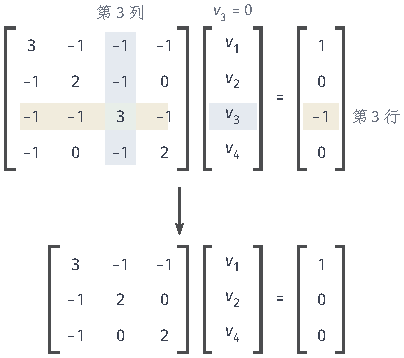
\includegraphics[scale=1]{figures/03-graphs/05-matrices-and-spectra/tikz/electrical-grounded-matrix/figure.pdf}
  \caption{在顶点$3$接地。上方是四点网络的全系统，蓝色竖带标出乘$v_3$的一列，黄色横带标出顶点$3$的方程。约化系统保留顶点$1,2,4$的未知量和守恒式。}
  \label{fig:electrical-grounded-matrix}
\end{BookInlineFigure}

\begin{figure}[!htb]
\centering
\begin{tikzpicture}[x=1mm,y=1mm,>=Stealth,
  vertex/.style={circle,draw=FigureBlue,fill=FigureBlueFill,inner sep=0pt,
    minimum size=5.5mm,line width=.52pt,font=\figurefont\fontsize{8}{10}\selectfont},
  gnd/.style={vertex,fill=FigureBlueFill,draw=FigureBlue,line width=.72pt},
  inject/.style={vertex,fill=FigureYellowFill,draw=FigureYellow,line width=.72pt},
  elabel/.style={font=\figurefont\fontsize{7}{8.5}\selectfont,FigureInk},
  vlabel/.style={font=\figurefont\fontsize{7.5}{9}\selectfont,FigureInk},
  panel/.style={anchor=mid,font=\figurefont\footnotesize}]
  % Left: setup
  \begin{scope}[xshift=0mm]
    \node[inject] (l1) at (0,14) {$1$};
    \node[vertex] (l2) at (14,14) {$2$};
    \node[gnd]    (l3) at (14,0) {$3$};
    \node[vertex] (l4) at (0,0) {$4$};
    \draw[FigureStroke,line width=.45pt] (l1)--(l2) (l2)--(l3) (l3)--(l4) (l4)--(l1) (l1)--(l3);
    \draw[->,FigureYellow,line width=.8pt] (-6,14) -- (l1) node[vlabel,midway,above] {$+1$};
    \draw[->,FigureBlue,line width=.8pt]  (l3) -- (20,0) node[vlabel,midway,above] {$-1$};
    \node[vlabel,below=1mm] at (l3.south) {接地};
    \node[panel] at (7,-8) {(a) 注入与接地};
  \end{scope}
  % Arrow
  \draw[->,FigureStroke,line width=.7pt] (26,7) -- (38,7) node[midway,above,font=\figurefont\fontsize{7}{8.5}\selectfont] {求解};
  % Right: solution
  \begin{scope}[xshift=44mm]
    \node[inject] (r1) at (0,14) {$1$};
    \node[vertex] (r2) at (14,14) {$2$};
    \node[gnd]    (r3) at (14,0) {$3$};
    \node[vertex] (r4) at (0,0) {$4$};
    \draw[FigureStroke,line width=.45pt] (r1)--(r2) (r2)--(r3) (r3)--(r4) (r4)--(r1) (r1)--(r3);
    \node[vlabel,left=1.5mm] at (r1) {$\frac{1}{2}$};
    \node[vlabel,right=1.5mm] at (r2) {$\frac{1}{4}$};
    \node[vlabel,right=1.5mm] at (r3) {$0$};
    \node[vlabel,left=1.5mm] at (r4) {$\frac{1}{4}$};
    % Current arrows
    \draw[->,FigureBlue,line width=.65pt] ([xshift=.5mm,yshift=-1mm]r1.east) -- ([xshift=-.5mm,yshift=-1mm]r2.west) node[elabel,above=.5mm,midway] {$\frac{1}{4}$};
    \draw[->,FigureBlue,line width=.65pt] ([xshift=-1mm,yshift=.5mm]r2.south) -- ([xshift=-1mm,yshift=-.5mm]r3.north) node[elabel,left=.5mm,midway] {$\frac{1}{4}$};
    \draw[->,FigureBlue,line width=.65pt] ([xshift=1mm,yshift=.5mm]r4.north) -- ([xshift=1mm,yshift=-.5mm]r1.south) node[elabel,right=.5mm,midway] {$\frac{1}{4}$};
    \draw[->,FigureBlue,line width=.65pt] ([xshift=.5mm,yshift=1mm]r3.west) -- ([xshift=-.5mm,yshift=1mm]r4.east) node[elabel,below=.5mm,midway] {$\frac{1}{4}$};
    \draw[->,FigureBlue,line width=.85pt] ([xshift=1.5mm,yshift=-1.5mm]r1.south east) -- ([xshift=-1.5mm,yshift=1.5mm]r3.north west) node[elabel,above right=0mm,midway] {$\frac{1}{2}$};
    \node[panel] at (7,-8) {(b) 电势与电流};
  \end{scope}
\end{tikzpicture}
\caption{四点电网络的接地求解。(a) 在顶点$1$注入$1$单位电流（浅黄），在顶点$3$接地（浅蓝）并引出$1$单位。(b) 求解后的电势标在顶点旁，蓝色箭头和数值给出实际电流方向及大小。对角边承载$1/2$的电流，两条外侧支路各承载$1/4$。}
\label{fig:electrical-grounding-overview}
\end{figure}

\begin{figure}[htbp]
  \centering
  \begin{tikzpicture}[
  figure picture,
  terminal/.style={circle,draw=FigureStroke,fill=FigureModelFill,
    minimum size=7mm,inner sep=0pt,line width=.75pt},
  conductor/.style={figure flow},
]
  \node[terminal] (v1) at (-2.3,0) {$1$};
  \node[terminal] (v2) at (0,1.3) {$2$};
  \node[terminal] (v3) at (2.3,0) {$3$};
  \node[terminal] (v4) at (0,-1.3) {$4$};

  \draw[conductor] (v1) -- node[figure edge label,above left] {$1/4$} (v2);
  \draw[conductor] (v2) -- node[figure edge label,above right] {$1/4$} (v3);
  \draw[conductor] (v1) -- node[figure edge label,below left] {$1/4$} (v4);
  \draw[conductor] (v4) -- node[figure edge label,below right] {$1/4$} (v3);
  \draw[conductor] (v1) -- node[figure edge label,above] {$1/2$} (v3);

  \node[left=4pt of v1] {$v_1=1/2$};
  \node[above=4pt of v2] {$v_2=1/4$};
  \node[right=4pt of v3] {$v_3=0$};
  \node[below=4pt of v4] {$v_4=1/4$};
\end{tikzpicture}

  \caption{四点环加对角边的电流分配。各边电导为一，顶点$1$注入一单位电流，顶点$3$接地并引出一单位。节点旁标注电势，边上箭头和数值给出实际电流方向及大小。两条外侧支路各输送$1/4$，中间支路输送$1/2$。}
  \label{fig:electrical-current-split}
\end{figure}

\subsection{一般网络的数值求解}
\label{sec:electrical-numerical-solve}

对于一般的连通电网络，接地后的约化方程组$\overline{\bm L}\,\overline{\bm v} = \overline{\bm b}$是一个$(n-1)$阶对称正定线性方程组，不接地时在正交补子空间$\bm 1^\perp$上求最小范数解$\bm v_{\mathrm{zm}}=\bm L^\dagger\bm b$则是对称半正定相容方程组的求解问题。因此，\BookChapterRef{part:linear-equations-optimization}{卷二第三部分“线性方程与优化”}中建立的各类线性方程组求解方法均可直接应用于电网络求解。

首先是直接分解法（详见\BookChapterRef{chap:direct-linear-solvers}{卷二“线性方程的直接求解”章}），如LU分解、对称正定矩阵的Cholesky分解$\overline{\bm L}=\bm G\bm G^\top$或分块$\bm L\bm D\bm L^\top$分解，在精确算术下通过前代与回代于有限步内求出电势；浮点实现还需控制舍入误差。当图结构与接地点固定而需对多个注入右端$\overline{\bm b}$反复求解时，三角因子可重复使用；但在稀疏图上消去内部顶点$i$会使它的所有邻居两两产生新的非零耦合项（即消元填充现象，见图~\ref{fig:electrical-cholesky-fill-in}），实际存储与计算开销取决于消元顺序下的填充边数量。

其次是定常迭代法（详见\BookChapterRef{sec:ls-stationary-iterations}{卷二“定常迭代法”章}）与行列投影法（详见\BookChapterRef{sec:ls-row-projection}{卷二“行列投影迭代法”章}），如Richardson、Jacobi、Gauss--Seidel、逐次超松弛（SOR/SSOR）或Kaczmarz投影法，仅通过局部邻域电势更新逐步逼近平衡电势，无需改动原图的稀疏结构。

再者是Krylov子空间法与预条件技术（详见\BookChapterRef{chap:krylov-methods}{卷二“Krylov子空间法”章}），如共轭梯度法（CG）、最小残差法（MINRES）与预条件共轭梯度法（PCG）。每步迭代的核心运算只需遍历全部$m$条边计算一次稀疏矩阵向量乘法$\bm x\mapsto\bm L\bm x$（耗时$O(n+m)$）；对条件数为$\kappa=\kappa_2(\bm A)$的正定系统$\bm A\bm x=\bm d$，共轭梯度法第$k$步能量范数误差满足
\begin{equation}
  \lVert\bm e^{(k)}\rVert_{\bm A}
  \leq 2\left(\frac{\sqrt\kappa - 1}{\sqrt\kappa + 1}\right)^k
  \lVert\bm e^{(0)}\rVert_{\bm A}.
  \label{eq:electrical-cg-error}
\end{equation}
至于直接法与各类迭代法在误差控制与总计算成本上的权衡选择，可参见\BookChapterRef{chap:solution-error-regularization}{卷二“求解误差、正则化与方法选择”章}；第~\ref{chap:graph-sparsification}章还将专门讨论如何用图的谱稀疏化构造拉普拉斯预条件子。

\begin{BookInlineFigure}
  \centering
  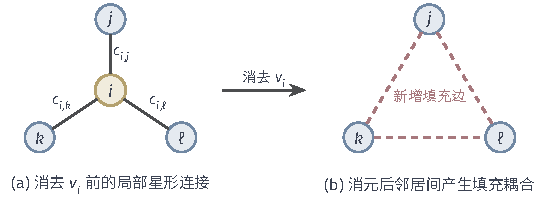
\includegraphics[width=92.385mm]{figures/03-graphs/05-matrices-and-spectra/tikz/electrical-cholesky-fill-in/figure.pdf}
  \caption{稀疏电网络直接消元中的填充现象。（a）消去顶点$i$之前，$i$与三个彼此不相邻的邻居$j,k,\ell$呈星形连接。（b）消去$v_i$后，邻居$j,k,\ell$之间两两产生新的非零耦合项（红色虚线填充边）。}
  \label{fig:electrical-cholesky-fill-in}
\end{BookInlineFigure}

\subsection{树上的线性时间求解}
\label{sec:electrical-tree-solve}

当电网络的正权支撑是一棵树$T=(V,E)$（边数$m=n-1$）时，图中不存在环路；按叶节点到根的顺序消元不会产生填充，任意消元顺序则未必如此。利用树的无环结构，无需显式构造矩阵，只需通过“自底向上求边电流、自顶向下求顶点电势”的两遍树遍历，就能在$O(n)$线性时间内精确解出拉普拉斯方程$\bm L\bm v=\bm b$。

先推导树上边电流与子树注入量的直接关系。任选顶点$q\in V$作为树的根（并令其为接地点$v_q=0$）。对每个非根顶点$i\neq q$，记$p(i)$为其父顶点，并将连接$i$与$p(i)$的唯一树边定向为从子指向父：$e_i\colon i\to p(i)$。删去树边$e_i$会将整棵树恰好切分为两部分：以$i$为根的子树$T_i$，以及包含根$q$的其余部分$V\setminus T_i$。

将子树$T_i$内部所有顶点$u\in T_i$的Kirchhoff电流守恒方程相加：子树内部的每一条边两个端点都在$T_i$内，其电流在尾端贡献正值、在头端贡献负值，正负成对抵消；唯一一条一端在$T_i$内、另一端在$T_i$外（即父顶点$p(i)$）的边界边正是$e_i\colon i\to p(i)$。因此，从$i$流向父顶点$p(i)$的边电流$s_i = f_{i\to p(i)}$必然精确等于整棵子树$T_i$内部的外部注入总和：
\begin{equation}
  s_i = \sum_{u\in T_i} b_u = b_i + \sum_{j\colon p(j) = i} s_j\qquad (i\neq q).
  \label{eq:electrical-subtree-injection}
\end{equation}

有了每条树边上的电流$s_i$后，再沿每条边$i\to p(i)$应用Ohm定律$s_i = c_{i,p(i)}(v_i - v_{p(i)})$，即可由父顶点的电势$v_{p(i)}$直接递推算出子顶点$i$的电势：
\begin{equation}
  v_i = v_{p(i)} + r_{i,p(i)}\,s_i\qquad (i\neq q),
  \label{eq:electrical-tree-voltage}
\end{equation}
其中$r_{i,p(i)} = 1/c_{i,p(i)}$为该树边的电阻。

据此，树上拉普拉斯方程$\bm L\bm v=\bm b$的$O(n)$求解算法完整流程如下（图~\ref{fig:electrical-tree-two-pass}）：

\paragraph{第一阶段：定根与父子序构建}
以接地点$q$为根，从$q$出发作一次广度优先或深度优先搜索，确定每个非根顶点$i\neq q$的父顶点$p(i)$及子节点列表，并按从根到叶的顺序记录遍历序列$(u_1=q, u_2, \ldots, u_n)$（父节点始终排在子节点之前）。

\paragraph{第二阶段：自底向上汇总子树注入求边电流（子节点先于父节点）}
按序列的逆序$u_n, u_{n-1}, \ldots, u_1$（即从叶子向根的自底向上顺序，此时处理顶点$i$时其所有子节点$j$的$s_j$均已算出）依次计算式~\eqref{eq:electrical-subtree-injection}：
\[
  s_i \leftarrow b_i + \sum_{j\colon p(j)=i} s_j.
\]
对叶节点，求和为空，直接有$s_i = b_i$；对内部节点$i\neq q$，算出的$s_i$即为边$i\to p(i)$上的电流。到达根节点$q$时，算出$s_q = \sum_{u\in V}b_u$：若$s_q\neq 0$，则外部注入总和不为零，报告方程组无解并终止；若$s_q = 0$，进入第三阶段。

\paragraph{第三阶段：自顶向下累加压降恢复顶点电势（父节点先于子节点）}
固定根节点电势$v_q \leftarrow 0$。按正序$u_2, \ldots, u_n$（即从根向叶的自顶向下顺序，此时处理顶点$i$时其父电势$v_{p(i)}$已经算出）依次由式~\eqref{eq:electrical-tree-voltage}计算
\[
  v_i \leftarrow v_{p(i)} + r_{i,p(i)}\,s_i.
\]
遍历结束即得全部顶点的唯一接地电势向量$\bm v$与全部树边的电流（若原边参考方向为$p(i)\to i$，只需将该边电流取为$-s_i$）。三个阶段均只对每个顶点和每条树边访问常数次，总时间复杂度和空间复杂度均为$O(n)$。

\begin{BookInlineFigure}
  \centering
  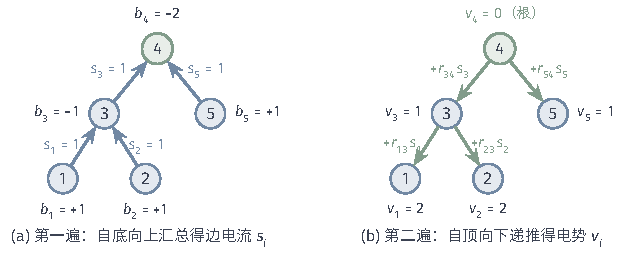
\includegraphics[width=105.174mm]{figures/03-graphs/05-matrices-and-spectra/tikz/electrical-tree-two-pass/figure.pdf}
  \caption{五顶点单位电阻树（以顶点$4$为根，注入$\bm b=(1,1,-1,-2,1)^\top$）上的两遍线性时间求解过程。（a）第一遍自底向上（从叶向根）按$s_i=b_i+\sum_{j:p(j)=i}s_j$汇总子树注入，直接定出每条边指向父节点的电流$s_1=1,s_2=1,s_3=-1+1+1=1,s_5=1$。（b）第二遍自顶向下（从根$v_4=0$向叶）按$v_i=v_{p(i)}+r_{i,p(i)}s_i$逐层累加压降，算出各点电势$v_3=1,v_5=1,v_1=2,v_2=2$。}
  \label{fig:electrical-tree-two-pass}
\end{BookInlineFigure}

以图~\ref{fig:electrical-tree-two-pass}中的五顶点单位电阻树（$r_e=1$）核对算法过程：设根为$4$，顶点$3$和$5$以$4$为父，叶子$1$和$2$以$3$为父，外部注入为$\bm b=(1,1,-1,-2,1)^\top$。

第一遍自底向上：叶子$1,2,5$直接取自身注入，得$s_1=1$、$s_2=1$、$s_5=1$；内部顶点$3$汇总自身注入$b_3=-1$与两个子节点的$s_1,s_2$，得$s_3 = -1 + 1 + 1 = 1$；根$4$处汇总得$s_4 = b_4 + s_3 + s_5 = -2 + 1 + 1 = 0$，守恒条件满足。

第二遍自顶向下：令根电势$v_4 = 0$；第一层子节点电势为$v_3 = v_4 + 1\times s_3 = 1$、$v_5 = v_4 + 1\times s_5 = 1$；第二层叶子电势为$v_1 = v_3 + 1\times s_1 = 2$、$v_2 = v_3 + 1\times s_2 = 2$，即得唯一接地电势解$\bm v=(2,2,1,0,1)^\top$。
